\section{Results}
We tested this model using two simulation scenarios and one real data set. The simulations include both
uniquely-labelled trees, to allow for comparison with traditional pairwise distance-based methods, as well as
genome-level simulation scenarios, leading to mul-trees.

For the first simulation scenario, starting from a random tree T0 on n leaves, we applied a series of consecutive SPR
branch swapping, storing all resulting trees  ${Ti} (0 \leq i leq N)$.  
As a result we know that Ti  and Ti-1 disagree by only
one SPR, Ti  and Ti-2 by two SPRs, etc., neglecting cases where the branch swappings cancel each other out. Therefore we
can use their relative location in this series (the ‘SPR chain’) as an indicator of their dissimilarity. We collected
them into 4 sets of 10 consecutive trees each to serve as our sample gene trees, separated by <y> trees – some of which
were used as reference trees. To test the effect of missing data we randomly removed leaves from each sample tree, such
that trees belonging to the same ‘group’ (i.e. consecutives in our chain of trees) have the same leaves removed. Only
the sample trees have missing leaves, but not the reference trees (by design of our model). [ Both the sample trees
(representing gene trees) and the reference trees (representing species trees) belong to the chain, but only the sample
trees have missing leaves. ]

The results are shown in figure 2, where we compare the effect of using reference trees belonging to the SPR chain (i.e.
similar to the sample trees in an SPR sense) or using randomly selected reference trees on the metric multidimensional
scaling (MDS) projection of the trees. We can conclude that choosing carefully the reference trees (i.e. that are close
to the samples) can help separating the sample gene family trees, even when these sample trees have missing data. On the
other hand using random trees did not seem to compromise the overall separation between groups. In this simulation
scenario all gene tree pairs can be directly compared since we do not have mul-trees (each species is uniquely
represented in the gene family tree), and therefore can be compared using distance matrix-based models (Gori et al.
2016). We therefore used our library to emulate the behaviour of treeCL (Gori et al. 2016) but using the approximate SPR
distance in addition to the RF distance, normalised to account for the unequal number of leaf comparisons. Pairwise
distance matrices creating using both measures provided MDS coordinates comparable to our tree signal using good
reference trees (results not shown). 


\begin{figure}[!htbp]
\begin{minipage}{7in}\centering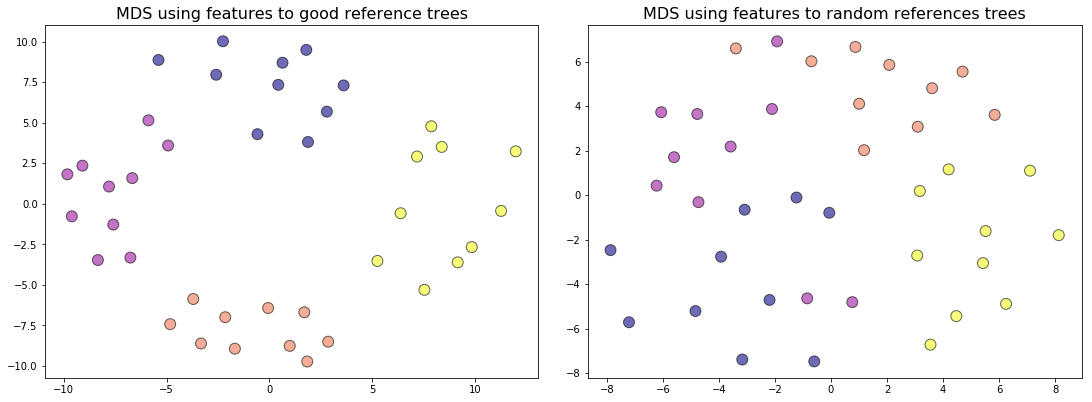
\includegraphics[width = 6.5in]{figure002.png}\end{minipage}
\caption{\label{figure002}
 SPR chain simulation with missing data. On the left panel we see the MDS projections of the samples when their signal
 is calculated from similar reference trees, and on the right we have the projections when random species trees are
 used. The colors represent the four groupings (consecutive trees in the SPR chain, separated from each other by more
 SPR branch swappings) defined in the simulation. 
}\end{figure}


The second simulation scenario was based on a genome-level simulation, where the gene trees are simulated , using the
software Simphy (Mallo, de Oliveira Martins, and Posada 2015), according to the multispecies coalescent within a locus
tree, which is generated under a duplication-loss model from a species tree. We generated 4 species trees with 20
species and from each species tree we simulated 50 gene families, assuming randomly between one or two genomes from each
species (simulating the sampling process of populations under the coalescent). Finally we removed up to half the leaves
from each gene family, and we used 116 trees similar to the true species trees as reference trees --- generated by random
branch swapping on the original ones.

There are many parameters controlling Simphy (from the multispecies coalescent to the birth-death process), and for most
of them we let the software sample from distributions, in order to allow for heterogeneity between gene families. We
tried several such combinations and show here a typical case, based on the observed distribution of leaves and species
per gene family tree, and where a bit less than half the species are common to gene family pairs. The parameters chosen
led to an expectation of one duplication and one loss per branch of the species tree, with 0.2 expected horizontal gene
transfers per branch, and moderate levels of incomplete lineage sorting. Parameter values more extreme led to large gene
families with less than half the species represented, and with very few (less than four) species in common per pair.

The result for a typical simulation is shown in figure 3, where we see that gene families from distinct species trees
can be discriminated.


\begin{figure}[!htbp]
\begin{minipage}{7in}\centering
  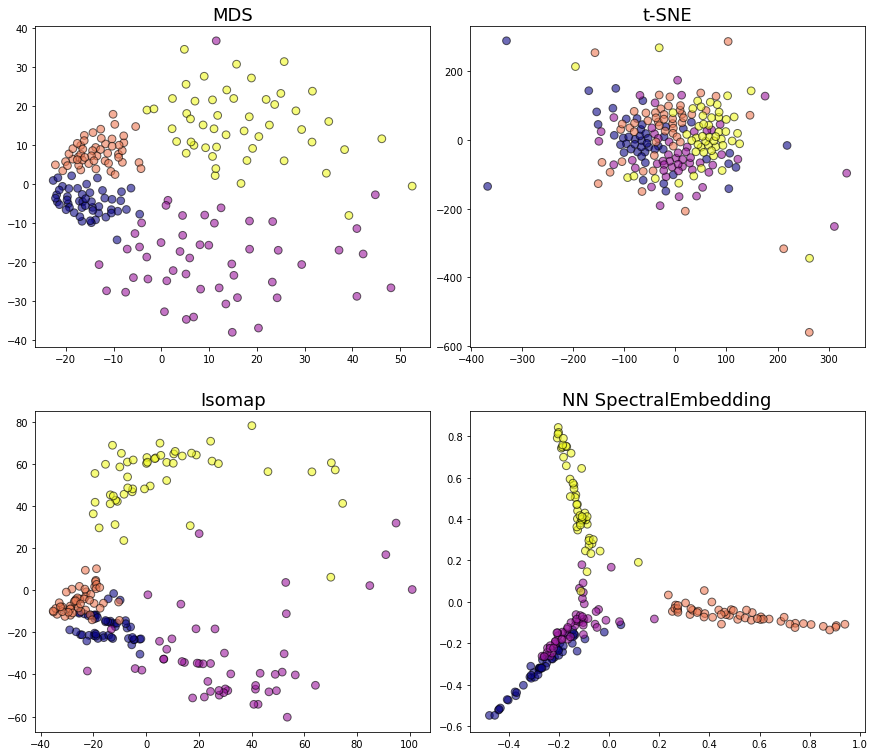
\includegraphics[width = 6in]{figure003a.png}
  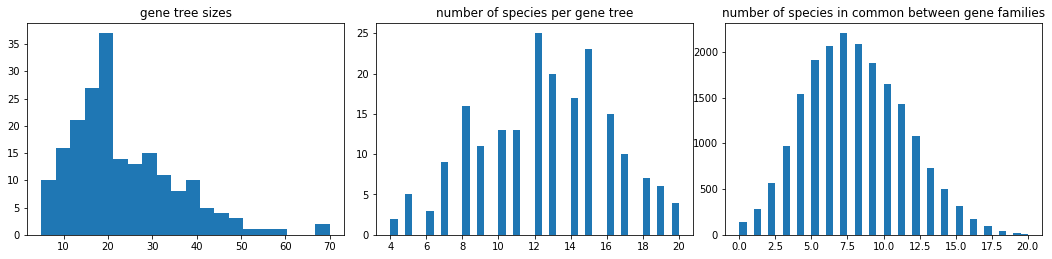
\includegraphics[width = 6in]{figure003b.png}
\end{minipage}
\caption{\label{figure003}
Typical case (simphy simulation). Colors represent underlying species trees.
}\end{figure}

\begin{figure}[!htbp]
\begin{minipage}{7in}\centering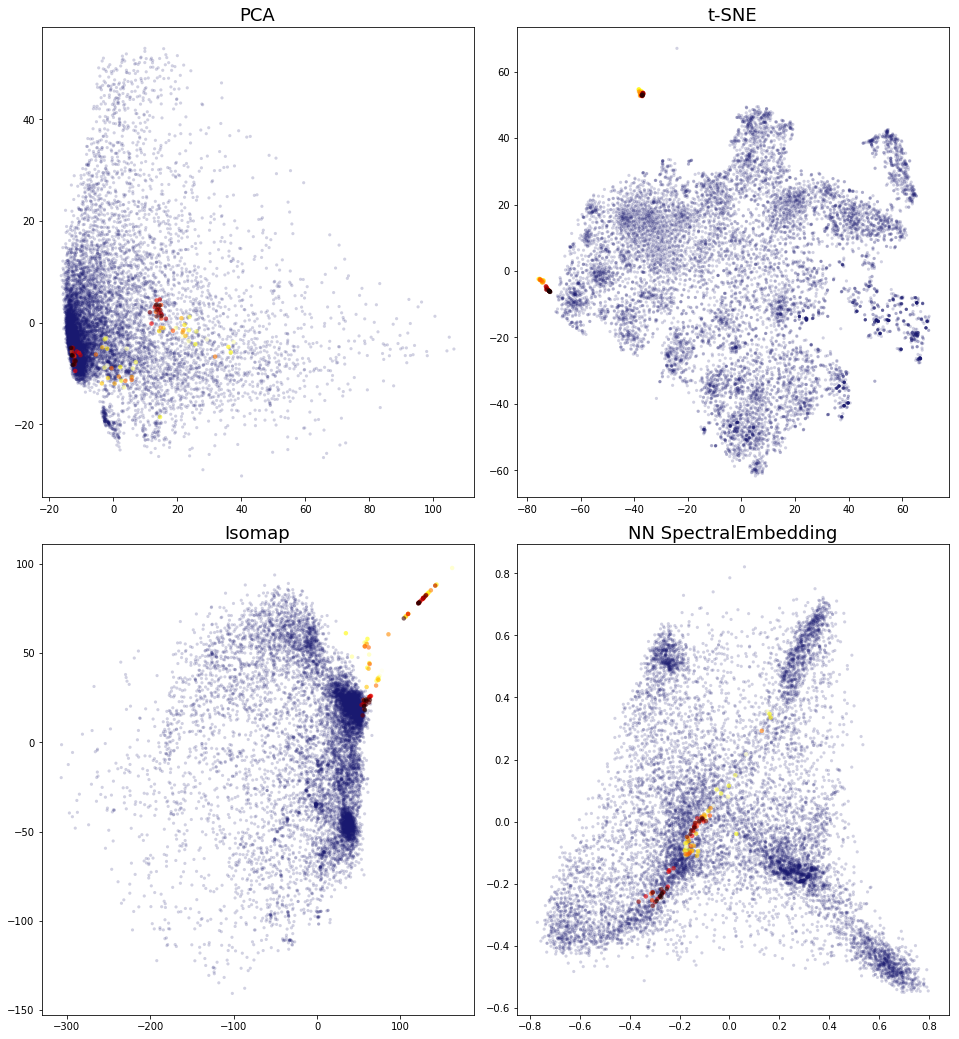
\includegraphics[width = 6.5in]{figure004.png}\end{minipage}
\caption{\label{figure004}
Fungal data set
}\end{figure}


